% ****** Start of file aipsamp.tex ******
%
%   This file is part of the AIP files in the AIP distribution for REVTeX 4.
%   Version 4.1 of REVTeX, October 2009
%
%   Copyright (c) 2009 American Institute of Physics.
%
%   See the AIP README file for restrictions and more information.
%
% TeX'ing this file requires that you have AMS-LaTeX 2.0 installed
% as well as the rest of the prerequisites for REVTeX 4.1
%
% It also requires running BibTeX. The commands are as follows:
%
%  1)  latex  aipsamp
%  2)  bibtex aipsamp
%  3)  latex  aipsamp
%  4)  latex  aipsamp
%
% Use this file as a source of example code for your aip document.
% Use the file aiptemplate.tex as a template for your document.
\documentclass[%
 aip,
 jmp,
 amsmath,
 amssymb,
%preprint,%
 reprint,%
%author-year,%
%author-numerical,%
 numerical,
 longbibliography,
]{revtex4-1}

\usepackage{graphicx}% Include figure files
\graphicspath{{images/}}
\usepackage{dcolumn}% Align table columns on decimal point
\usepackage{bm}% bold math
\usepackage{url}
\usepackage{float}
\usepackage{silence}
\usepackage{tabularx}
\WarningFilter{revtex4-1}{Repair the float}
%\usepackage[mathlines]{lineno}% Enable numbering of text and display math
%\linenumbers\relax % Commence numbering lines

\begin{document}

%\preprint{AIP/123-QED}

\title[Laboratory 1]{Inroduction to DC Measurements} % Force line breaks with \\

\author{Kevin "Yama" Keyser}
 \email{kk8r8@mail.umck.edu}
\affiliation{ 
	University of Missouri-Kansas City
	%\\This line break forced with \textbackslash\textbackslash
}%

%\date{\today}% It is always \today, today,
             %  but any date may be explicitly specified

\begin{abstract}
In Laboratory 1, we are introduced to the usages of the Digital Multimeter (DMM), and how
to apply it when measuring resistance, voltage, and current across a circuit.
We also learn the trace diagram for the Elenco breadboard (which the general idea
can be applied to other solderless breadboards).
\end{abstract}

%\keywords{Operational Amplifier}%Use showkeys class option if keyword
                              %display desired
\maketitle

%\begin{quotation}
%The ``lead paragraph'' is encapsulated with the \LaTeX\ 
%\verb+quotation+ environment and is formatted as a single paragraph before the first section heading. 
%(The \verb+quotation+ environment reverts to its usual meaning after the first sectioning command.) 
%Note that numbered references are allowed in the lead paragraph.
%
%The lead paragraph will only be found in an article being prepared for the journal \textit{Chaos}.
%\end{quotation}

\section{Background}

On a personal note, there was already a lot of familiarity with using DMMs, and solderless
breadboards before this lab. We will be applying Kirchhoff's laws for voltage and current
for some of the circuit we set up. One note to make is the sensitivity of the measuring
equipment. The only DMM that has a mA option, doesn't seem to work for the lower readings.
The fuse may be blown out on the DMM.

\section{Procedure}

The procedures for Laboratory 1 is very straight forward, so the Laboratory 1 sheet will be attached at the end of this write up.

\section{Presentation of Data}

	\subsection{1-1: Resistance Measurements}
	
	\begin{tabularx}{0.45\textwidth}[t]{| X | X | X |}
	\hline
	\multicolumn{3}{|c|}{Resistance Values vs Measure Values}\\
	\hline
		\multicolumn{1}{|c|}{Resistor} & 
		\multicolumn{1}{c|}{DMM} & 
		\multicolumn{1}{c|}{DMM while Held} \\ 
	\hline
	10 & 9.9 & 9.9\\ \hline
	105 & 105.1 & 105.1\\ \hline
	1k & 0.983k & 0.982k\\ \hline
	10k & 9.82k & 9.74k\\ \hline
	100k & 99.2k & 81.9k\\ \hline
	1M & 0.968M & 0.390M\\ \hline
	10M & 10.29M & 0.390M\\ \hline
	\end{tabularx}
	
	\begin{tabularx}{0.45\textwidth}[t]{| X | X | X | X |}
	\hline
	\multicolumn{4}{|c|}{Resistance When Heated}\\
	\hline
		\multicolumn{1}{|c|}{Type} &
		\multicolumn{1}{c|}{Listed Value} & 
		\multicolumn{1}{c|}{DMM} & 
		\multicolumn{1}{c|}{DMM (heated)} \\ 
	\hline
	Carbon & 10k & 9.83k & 9.65k\\ \hline
	Metal Film & 11k & 10.95k & 10.99k\\ \hline
	\end{tabularx}
	
	\subsection{1-2: Introduction to the breadboard frame}
	
	No tabular data. Will discuss experimental results in the Discussion section.
	
	\subsection{1-3: DC Voltage Measurement}
	
	\begin{tabularx}{0.45\textwidth}[t]{| X | X | X |}
	\hline
		\multicolumn{1}{|c|}{V Listing} & 
		\multicolumn{1}{c|}{V Actual} & 
		\multicolumn{1}{c|}{Breadboard Reading} \\ 
	\hline
	+5V & 5.045V & 5.045V\\ \hline
	+12V & 11.85V & 11.85V\\ \hline
	-12V & -12.11 & -12.11\\ \hline
	\end{tabularx}
	
	\subsection{1-4: Current Measurement}
	
	\begin{tabularx}{0.45\textwidth}[t]{| X | X | X |}
	\hline
	\multicolumn{2}{|c|}{Current Across Resistor} \\ 
	\hline
	\multicolumn{1}{|c|}{Voltage} & \multicolumn{1}{c|}{Current}\\ \hline
	8.45V & 0.009A\\ \hline
	10.76V & 0.011A\\ \hline
	\end{tabularx}
	
	\subsection{1-5: Meter Resistance}
	
	\begin{tabularx}{0.45\textwidth}[t]{| X | X |}
	\hline
	\multicolumn{2}{|c|}{Multimeter Resistance (Amps)} \\ 
	\hline
		\multicolumn{1}{|c|}{Without 10$\Omega$} & 
		\multicolumn{1}{c|}{With 10$\Omega$}\\ \hline
	.026A & .025A\\ \hline
	\end{tabularx}
	
	\subsection{1-6: Voltage Divider}		
	
	No tabular data. Will discuss experimental results in the Discussion section.
	
	\subsection{1-7: Resistors in Parallel}
	
	No tabular data. Will discuss experimental results in the Discussion section.
	
	\subsection{1-8: Complex Circuits}
	
	No tabular data. Will discuss experimental results in the Discussion section.
	
	\subsection{1-9: Charging a Capacitor}
	
	\begin{tabularx}{0.45\textwidth}[t]{| X | X |}
	\hline
	\multicolumn{2}{|c|}{Voltage Drop Across Capacitor} \\ 
	\hline
		\multicolumn{1}{|c|}{Time (s)} & 
		\multicolumn{1}{c|}{Voltage (mV)}\\ \hline
	0 & 1010\\ \hline
	5 & 920\\ \hline
	10 & 830\\ \hline
	15 & 765\\ \hline
	20 & 700\\ \hline
	25 & 635\\ \hline
	30 & 584\\ \hline
	35 & 535\\ \hline
	40 & 485\\ \hline
	\end{tabularx}

\section{Discussion} \label{Section:Discussion}

	\subsection{1-1: Resistance measurements}
	
	The resistors measured all fell within the tolerance listed each resistor (except the 
	968k$\Omega$ resistor. Their stamps suggest a $\pm$5\% tolerance. There will always be
	errors from the factory, and a decline in resistance over time. The body resistance 
	does seem to go down, the harder you press on the material/wire. This is easier to see
	with bigger valued resistors (1M$\Omega$ and 10M$\Omega$). This leads us to believe that
	the DMM uses current to measure resistance, since current will take the path of least
	resistance, which would make the body's resistance lower than those of the higher valued
	resistors.
	
	After heating 2 different resistors, there was an interesting effect. The carbon
	resistor's resistance went down, where the thin metal film one went up. This might make
	sense when taking into account that conductivity goes down for conductors. Since metals
	are conductors, the thin metal film's conductivity will go down, making its resistance
	actually go up.
	
	\subsection{1-2: Introduction to the Breadboard Frame}
	
	\begin{figure}[H]
	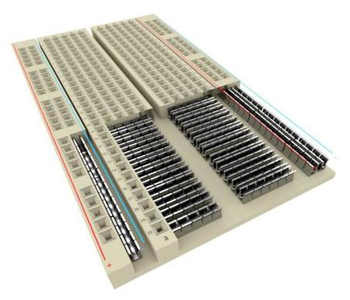
\includegraphics[width=\columnwidth]{BreadboardInternal.eps}
	\caption{\label{fig1}Open view of a breadboard.}
	\end{figure}
	
	There is not much to say here that the image can't convey. You have rows of solderless
	connectors, which are separated by a divider. Running along the sides of these connectors
	are voltage/ground rails. They're all just rows of metal that make it easier to prototype
	your connections. The resistance across the terminals/tie in points were virtually zero.
	
	\subsection{1-3: DC Voltage Measurement}
	
	This experiment, similar to the previous, was to show which points connected together, and
	to show the virtually zero resistance of these connections. The voltage in always equaled
	the voltage out. We would need a much more sensitive measuring device to see any change.
	
	\subsection{1-4: Current Measurements}
	
	There is one key thing to realize here: when using the DMM as an Ammeter, the current
	has to flow through the DMM. If you connect the DMM to the positive and negative (or 
	positive and ground), you will short the circuit. This is due to the low internal
	resistance of the DMM, and back to the first experiment, we know that current will want
	to travel through the path of least resistance (as will all things that flow). This is
	what is meant by a short. We will see in the next experiment, just how low the internal
	resistance of the DMM is. 
	
	The current does follow Ohm's law, but we don't know how exact. Our instruments are not
	sensitive enough to get a precise measure on it. The power supply will have its own
	internal resistance as well. This is why when doing calculations, when ignoring this,
	we call the battery an "`ideal"' battery. In real life, nothing is ideal, but we can
	pretend that for really low values, that they have a negligible effect.	
	
	\subsection{1-5: Meter Resistance}
	
	The first parts of this experiment uses the ideas behind Kirchhoff's Voltage Law.
	We see that the voltage across the 1M$\Omega$ resistor is the same as the voltage
	supplied. This is because the voltage supplied, minus all the voltage drops across
	each resister, should equal zero. Or mathematically:
	\[ V_s-V_1-V_2-\dots-V_n=0 \]
	Where 1, 2, $\dots$, n are resistors in series in the circuit.
	
	When we measure before the resistor, with respect to ground, we get or full voltage
	reading, but measuring after the resistor, we get zero. This is because since there
	is only one resistor in the circuit (ignoring the internal resistance of our power
	supply), all of the voltage drop will be across that resistor.
	
	Following that, we then have a circuit that is in parallel, and we find an addition
	to Kirchhoff's Voltage Law. The law applies to each loop in a circuit. Meaning, if
	resistors are placed in parallel, they should all experience the same voltage drop
	across each one. Said more mathematically:
	\[ V_s = V_1 = V_2 = \dots = V_n \]
	Similarly, where 1, 2, $\dots$, n are the resistors in parallel in the circuit.
	
	Then the final circuit, applying Kirchhoff's laws, should give us the internal
	resistance of the DMM. We made a small change here, and used a 200$\Omega$ resistor
	for our resistor from the power supply instead of a 1k$\Omega$ resistor, to make
	it easier to measure the differences. As expected, our value without the 10$\Omega$
	resistor is 26mA. Though our input is 5V (actually 5.045V) and our resistor is 
	200$\Omega$, there is a tolerance rating, so the calculation of Ohm's law is still
	within the bounds. Now, with the 10$\Omega$ resistor in parallel, we get a reading 
	of 25mA. Qualitatively put, this means that our DMM in Amp mode has an incredibly
	low resistance, if majority of the current in the circuit is still flowing through
	the DMM. It also means that our resistance is so low, that the equivalent resistance
	of the two resistors combined (see next subsection for formula) gives us almost the same
	total resistance in the circuit. Quantitatively, this means the DMM in Amp mode has
	an internal resistance of $\leq 1\Omega$.
	
	\subsection{1-6, 7, 8: Series, Parallel, and a combination}
	
	As stated above, we were unable to get accurate readings in the mA and below range,
	due to the only DMM in the lab that has an accuracy in the mA not seeming to work
	(most likely, the fuse on that side has been blown out).
	
	What we can deduce for the law of resistors from Kirchhoff's Voltage Law and our
	measurements goes as follows. We saw that in a series circuit, the current across
	all resistors stayed the same, but the voltage across all resistors is not. If we
	take the voltage across each resistor, and divide that by the resistor's value, we
	get the current. So for a circuit in series, we have
	\[ I_t = I_1 = \dots = I_n \]
	Further, because the total voltage drop across each should equal the voltage of our
	power supply, then the total voltage divided by the total resistance, equals our
	current. Looking at these values, we see that when resistors are in series, we get
	the formula
	\[ R_T = R_1 + R_2 + \dots + R_n \]
	
	Moving along to parallel circuits, doing the same analysis of voltage, and current, 
	and applying Kirchhoff's Current Law, we get the following formula for total/effective
	resistance for resistors in parallel
	\[ R_T = [\frac{1}{R_1} + \frac{1}{R_2} + \dots + \frac{1}{R_n}]^{-1}\]
	
	\subsection{1-9: Charging a Capacitor}
	
	\begin{figure}[H]
	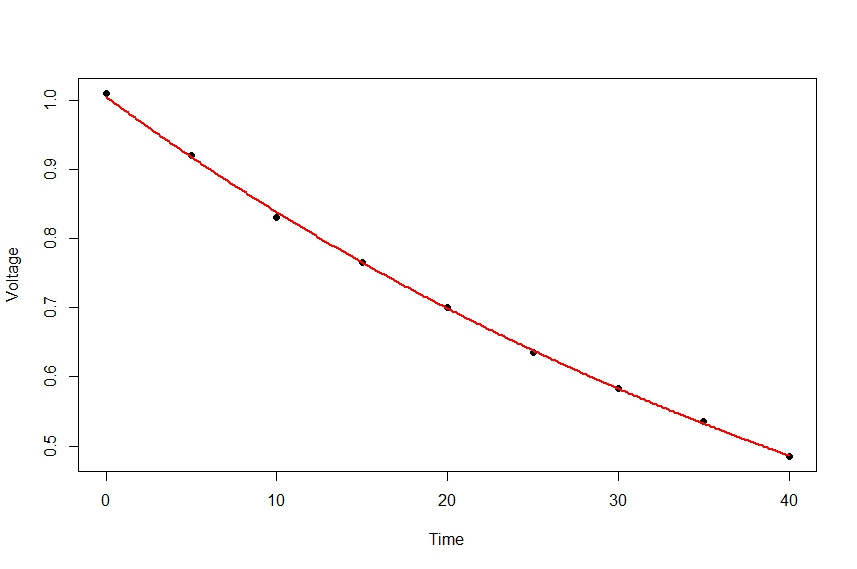
\includegraphics[width=\columnwidth]{ExponentialFit.eps}
	\caption{Fitting our data to an exponential curve in R.}
	\end{figure}
	
	Looking at the fit above, with an R-squared value of 0.9996, we can see that our values
	do follow an exponential decay, with most of the error being due to the limits of the 
	human brain and eye being able to read constantly falling values on a DMM (still, an
	R-squared value of 0.9996 is pretty amazing).

\section{Conclusion}

Though we were limited on the accuracy of the devices we had available to us, the overall
idea of the application of Kirchhoff's laws, and deriving them from what we observed in
our experiments was key. We were able to also figure out how to derive equivalent resistance
in a series and parallel circuit just from our observations. Though we had the benefit of
hindsight, and years of progress, the key points do not change. Unlike other fields, where
many of the rules are agreed upon, or chosen (I'm looking at you, Axiom of Choice), the
models that we come up with in Physics rely completely on understanding, and measuring 
what happens in nature. It is not up to us to make the rules. It is up to scientists
(and specifically here, physicists) to observer nature, and understand its rules. Being
able to pull insight from the smallest of interactions, and building upon those intuitions
is how we continue to find progress (though, yes, luck doesn't hurt).

\end{document}